% =============================================================
%  Informe — Semana 1 (MIA-B | Aprendizaje profundo | UIDE)
%  Perceptrón Multicapa sobre OSMI Mental Health Survey
%  Grupo 5 — J. Quizamánchuro Fuel, G. Calahorrano Guayasamin, D. Perez Cedillo
%
%  Entrega final del cuatrimestre. Plantilla 2-col del Grupo 5
%  (consistente con Semana 2 y Semana 3). Compatible con tectonic / pdflatex.
% =============================================================
\documentclass[10pt,a4paper,twocolumn]{article}

\usepackage[utf8]{inputenc}
\usepackage[T1]{fontenc}
\usepackage[spanish,es-tabla]{babel}
\usepackage{lmodern}
\usepackage{microtype}

\usepackage[a4paper,margin=2cm,headheight=14pt,headsep=10pt,footskip=24pt]{geometry}
\setlength{\columnsep}{0.7cm}

\usepackage{booktabs}
\usepackage{array}
\usepackage{tabularx}
\usepackage{colortbl}
\usepackage{xcolor}
\usepackage{graphicx}
\usepackage{caption}
\usepackage{float}

\definecolor{tableheader}{HTML}{F5B041}
\definecolor{linkbox}{HTML}{D4E6F1}
\definecolor{linkboxborder}{HTML}{A9CCE3}
\definecolor{highlight}{HTML}{D4EFDF}

\captionsetup{font=small,labelfont={bf,sf},labelsep=colon,format=plain,justification=raggedright,singlelinecheck=false}
\addto\captionsspanish{\renewcommand{\tablename}{Cuadro}}

\usepackage{fancyhdr}
\pagestyle{fancy}
\fancyhf{}
\renewcommand{\headrulewidth}{0pt}
\renewcommand{\footrulewidth}{0pt}
\fancyhead[L]{\footnotesize\sffamily MIA-B $\,|\,$ Aprendizaje profundo $\,|\,$ Grupo 5 $\,|\,$ Ejercicio Práctico Clase 1}
\fancyfoot[L]{\footnotesize\sffamily Aprendizaje profundo}
\fancyfoot[C]{\footnotesize\sffamily Universidad Internacional del Ecuador}
\fancyfoot[R]{\footnotesize\sffamily Mayo, 2026 \quad \thepage--3}

\fancypagestyle{firstpage}{%
    \fancyhf{}
    \renewcommand{\headrulewidth}{0pt}
    \renewcommand{\footrulewidth}{0pt}
    \fancyhead[L]{\footnotesize\sffamily MIA-B $\,|\,$ Aprendizaje profundo $\,|\,$ Grupo 5 $\,|\,$ Ejercicio Práctico Clase 1}
    \fancyfoot[L]{\footnotesize\sffamily Aprendizaje profundo}
    \fancyfoot[C]{\footnotesize\sffamily Universidad Internacional del Ecuador}
    \fancyfoot[R]{\footnotesize\sffamily Mayo, 2026 \quad \thepage--3}
}

\usepackage[hidelinks]{hyperref}
\hypersetup{colorlinks=true, linkcolor=black, urlcolor=blue!60!black, citecolor=black}

\usepackage[most]{tcolorbox}
\newtcolorbox{codigofuente}{
    enhanced, colback=linkbox, colframe=linkboxborder,
    boxrule=0.4pt, arc=2pt,
    left=8pt, right=8pt, top=6pt, bottom=6pt,
    fontupper=\small,
}

\usepackage{titlesec}
\titleformat{\section}{\normalfont\large\bfseries\sffamily}{\thesection.}{0.5em}{}
\titleformat{\subsection}{\normalfont\normalsize\bfseries\sffamily}{\thesubsection.}{0.5em}{}
\titlespacing*{\section}{0pt}{1.1\baselineskip}{0.4\baselineskip}
\titlespacing*{\subsection}{0pt}{0.8\baselineskip}{0.3\baselineskip}

\usepackage{enumitem}
\setlist{nosep,leftmargin=1.4em}

\newcommand{\githuburl}{https://github.com/georgenton/UIDE-Aprendizaje-Profundo/blob/main/semana-1/notebook/MLP\_Mental\_Health\_Survey.ipynb}

\begin{document}

% =========================================================
%  ENCABEZADO
% =========================================================
\twocolumn[
\begin{@twocolumnfalse}
\thispagestyle{firstpage}
\vspace*{0.5em}

\noindent{\LARGE\bfseries\sffamily Perceptrón Multicapa para Predicción de Búsqueda de Tratamiento en Salud Mental\par}

\vspace{0.8em}
\noindent{\normalsize\textbf{J. Quizamánchuro Fuel}$^{a}$, G. Calahorrano Guayasamin$^{a}$ y D. Perez Cedillo$^{a}$}

\vspace{0.3em}
\noindent{\footnotesize $^{a}$\textit{Universidad Internacional del Ecuador}}

\vspace{0.2em}
\noindent{\footnotesize \textbf{Profesor:} J. Rodriguez Chivata}

\vspace{1.0em}
\end{@twocolumnfalse}
]

\begin{codigofuente}
\textbf{Código fuente}\\[2pt]
$\hookrightarrow$~\href{\githuburl}{Notebook del Proyecto en GitHub}
\end{codigofuente}

% =========================================================
%  1. CONTEXTUALIZACIÓN
% =========================================================
\section{Contextualización del problema}

Las plataformas digitales de salud mental enfrentan un reto operativo común: priorizar a quién acercarse primero entre miles de usuarios. Predecir con qué probabilidad una persona buscaría tratamiento profesional dado su contexto laboral y demográfico permite orientar acciones de psicoeducación dirigida sin reemplazar la evaluación clínica.

Este trabajo implementa un \textbf{Perceptrón Multicapa (MLP)} sobre la encuesta \textbf{OSMI 2014} (\textit{Open Sourcing Mental Illness}) — un dataset de 1.259 respuestas de trabajadores tech que reporta variables laborales (beneficios, políticas, apertura), demográficas (edad, género, autoempleo) y antecedentes (historia familiar, tratamiento previo).

\textbf{Tarea:} clasificación binaria.\\
\textbf{Variable objetivo:} \texttt{treatment} (Sí / No).\\
\textbf{Relevancia profesional:} aplicable directamente a flujos de triaje en plataformas SaaS de psicoeducación (caso de uso: Psico Platform, plataforma del responsable técnico del Grupo 5).\\
\textbf{Restricción ética declarada:} el modelo predice una \textit{intención declarada}, no un diagnóstico clínico — esta distinción es central para uso responsable.

% =========================================================
%  2. PREPARACIÓN DEL DATASET
% =========================================================
\section{Preparación y limpieza del dataset}

El dataset original presenta tres problemas conocidos que requirieron limpieza específica: (a) la columna \texttt{Age} contiene valores absurdos (negativos y $>$100) por error de captura; se filtró al rango plausible 18--80 años (8 filas eliminadas); (b) la columna \texttt{Gender} es texto libre con más de 40 variantes que se normalizaron a tres categorías (Male: 996, Female: 245, Other: 10); (c) las columnas \texttt{state, comments, Country, Timestamp} se descartaron por irrelevancia o alto porcentaje de nulos. Los valores faltantes restantes en variables categóricas se imputaron con la moda. Las variables categóricas se codificaron con one-hot encoding, resultando en un espacio de 44 features.

\begin{table}[H]
\centering
\caption{Ficha técnica resumida}
\label{tab:ficha}
\footnotesize
\renewcommand{\arraystretch}{1.15}
\begin{tabularx}{\columnwidth}{>{\bfseries}lX}
\rowcolor{tableheader}\textcolor{white}{\textbf{Atributo}} & \textcolor{white}{\textbf{Valor}}\\
Muestras tras limpieza        & 1.251 \\
Features (post one-hot)       & 44 \\
Distribución de clases        & 50,5\,\% Sí / 49,5\,\% No \\
División Train/Val/Test       & 875 / 188 / 188 (estratificada) \\
Normalización                 & \texttt{StandardScaler} (ajustado solo en train) \\
Semilla aleatoria             & SEED = 42 \\
\end{tabularx}
\end{table}

\textbf{Por qué tres conjuntos:} el conjunto de validación permite monitorear overfitting y aplicar \textit{early stopping} sin contaminar el conjunto de prueba. El test del 15\,\% se mantiene como caja cerrada y solo se abre al final para reportar métricas honestas de generalización.

% =========================================================
%  3. ARQUITECTURA
% =========================================================
\section{Arquitectura del MLP}

Se diseñó un MLP de tres capas ocultas en arquitectura tipo embudo (64 $\rightarrow$ 32 $\rightarrow$ 16 neuronas), con activación ReLU en capas ocultas y sigmoide en la capa de salida. La compresión progresiva fuerza al modelo a aprender representaciones más abstractas en cada capa.

\textbf{ReLU} se eligió como estándar moderno por su eficiencia y resistencia al \textit{vanishing gradient}. La \textbf{sigmoide} en la salida mapea a una probabilidad calibrada en $[0,1]$, compatible con \texttt{binary\_crossentropy}.

\textbf{Parámetros entrenables:} 5.505. \textbf{Optimizador:} Adam con \texttt{lr=1e-3} — combina momentum y RMSProp con adaptación interna del LR. \textbf{Batch size:} 32. \textbf{Épocas máximas:} 150, con criterio de detención específico por variante.

% =========================================================
%  4. EXPERIMENTO REGULARIZACIÓN
% =========================================================
\section{Experimento — Comparación de estrategias de regularización}

Se eligió regularización como eje de análisis complementario. La justificación es doble: con 1.251 muestras y 44 features post-encoding, la razón muestras/features $\approx 28$ ubica al modelo en zona conocida de alto riesgo de overfitting. Adicionalmente, en contextos de salud mental, un modelo sobreajustado que aprende correlaciones espurias del subgrupo de entrenamiento es peligroso al desplegarse en poblaciones distintas. Se entrenaron \textbf{cuatro variantes} manteniendo idéntica la arquitectura, optimizador, batch size y semilla (SEED=42):

\begin{table}[H]
\centering
\caption{Configuraciones de regularización evaluadas}
\label{tab:variantes}
\footnotesize
\renewcommand{\arraystretch}{1.2}
\begin{tabularx}{\columnwidth}{>{\bfseries}l l X}
\rowcolor{tableheader}\textcolor{white}{\textbf{Variante}} & \textcolor{white}{\textbf{Config}} & \textcolor{white}{\textbf{Mecanismo}}\\
Baseline       & ---            & Referencia para medir el efecto \\
L2             & $\lambda=0{,}01$  & Penaliza pesos grandes en el loss \\
Dropout        & rate=0,3       & Apaga 30\,\% de neuronas aleatoriamente \\
Early Stopping & paciencia=15   & Detiene si val\_loss no mejora \\
\end{tabularx}
\end{table}

\begin{figure}[H]
\centering
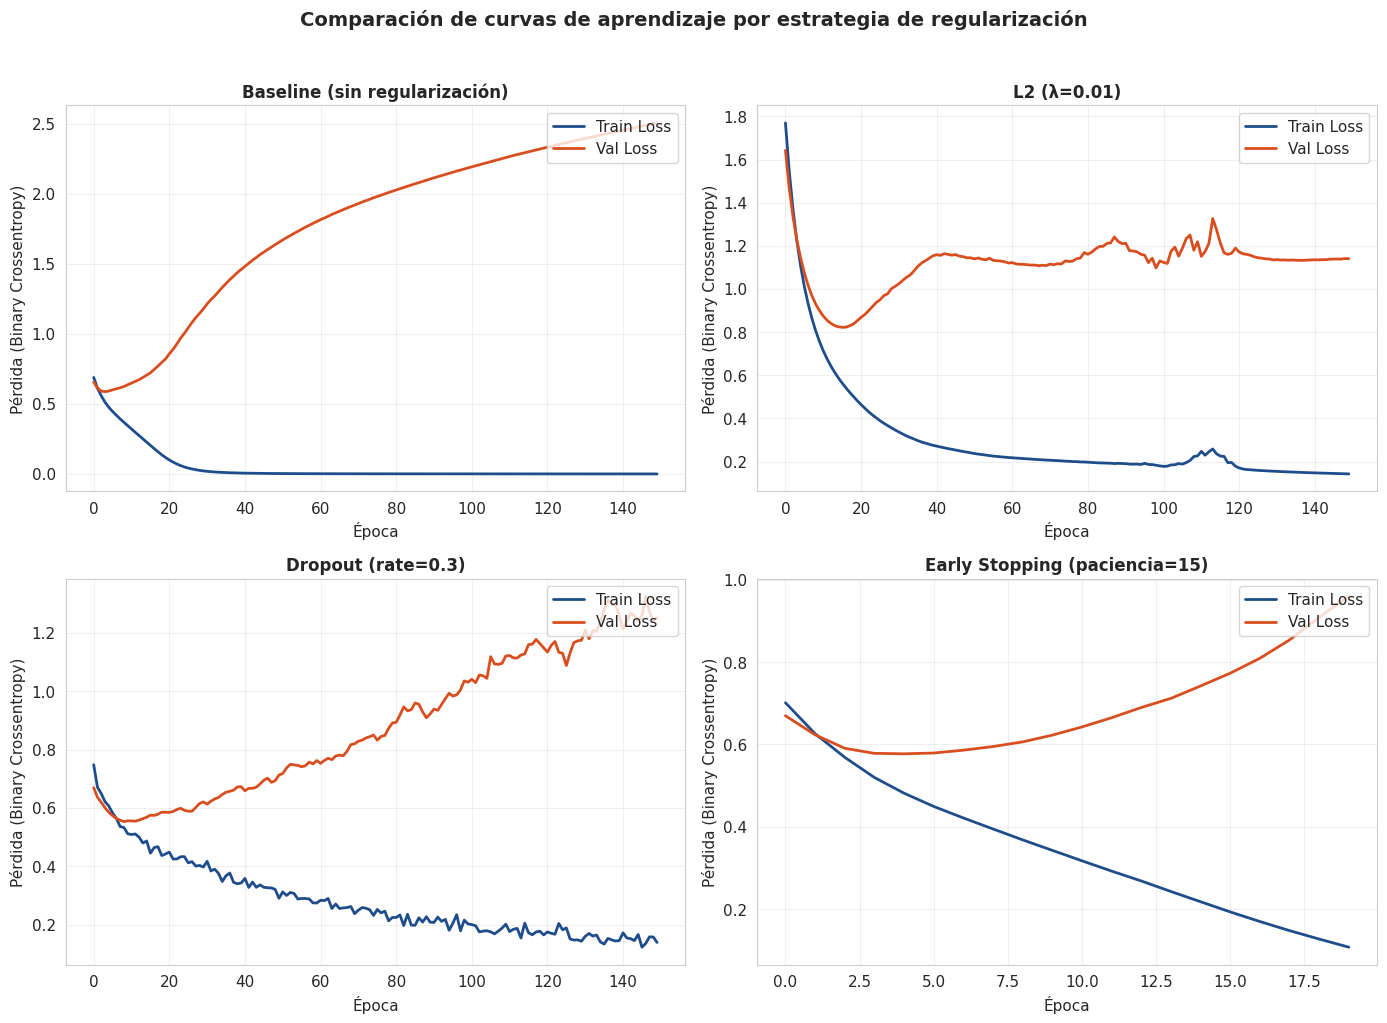
\includegraphics[width=\columnwidth]{figs/02_curvas_aprendizaje.png}
\caption{Curvas de aprendizaje por estrategia. El baseline muestra divergencia clara entre train y validation desde épocas tempranas (overfitting evidente). Las tres técnicas de regularización mantienen las curvas más cercanas. Early Stopping detuvo el entrenamiento tras 19 épocas; las otras variantes corrieron las 150 completas.}
\label{fig:curvas}
\end{figure}

% =========================================================
%  5. RESULTADOS
% =========================================================
\section{Resultados sobre conjunto de prueba}

Tras entrenar las cuatro variantes, se evaluó cada modelo sobre el conjunto de prueba (15\,\% reservado, n=188), nunca visto durante el entrenamiento ni el ajuste de hiperparámetros.

\begin{table}[H]
\centering
\caption{Métricas sobre conjunto de prueba. Verde = mejor modelo por F1.}
\label{tab:metricas}
\footnotesize
\renewcommand{\arraystretch}{1.25}
\begin{tabularx}{\columnwidth}{>{\bfseries}X c c c c c}
\rowcolor{tableheader}
\textcolor{white}{\textbf{Modelo}} & \textcolor{white}{\textbf{Acc.}} & \textcolor{white}{\textbf{Prec.}} & \textcolor{white}{\textbf{Rec.}} & \textcolor{white}{\textbf{F1}} & \textcolor{white}{\textbf{AUC}}\\
Baseline           & 0,6915 & 0,6947 & 0,6947 & 0,6947 & 0,7736 \\
L2 ($\lambda$=0,01) & 0,6755 & 0,6977 & 0,6316 & 0,6630 & 0,7393 \\
\rowcolor{highlight}
\textbf{Dropout (0,3)} & \textbf{0,7447} & \textbf{0,7527} & \textbf{0,7368} & \textbf{0,7447} & 0,7903 \\
Early Stopping     & 0,7553 & 0,8101 & 0,6737 & 0,7356 & \textbf{0,8222} \\
\end{tabularx}
\end{table}

\begin{figure}[H]
\centering
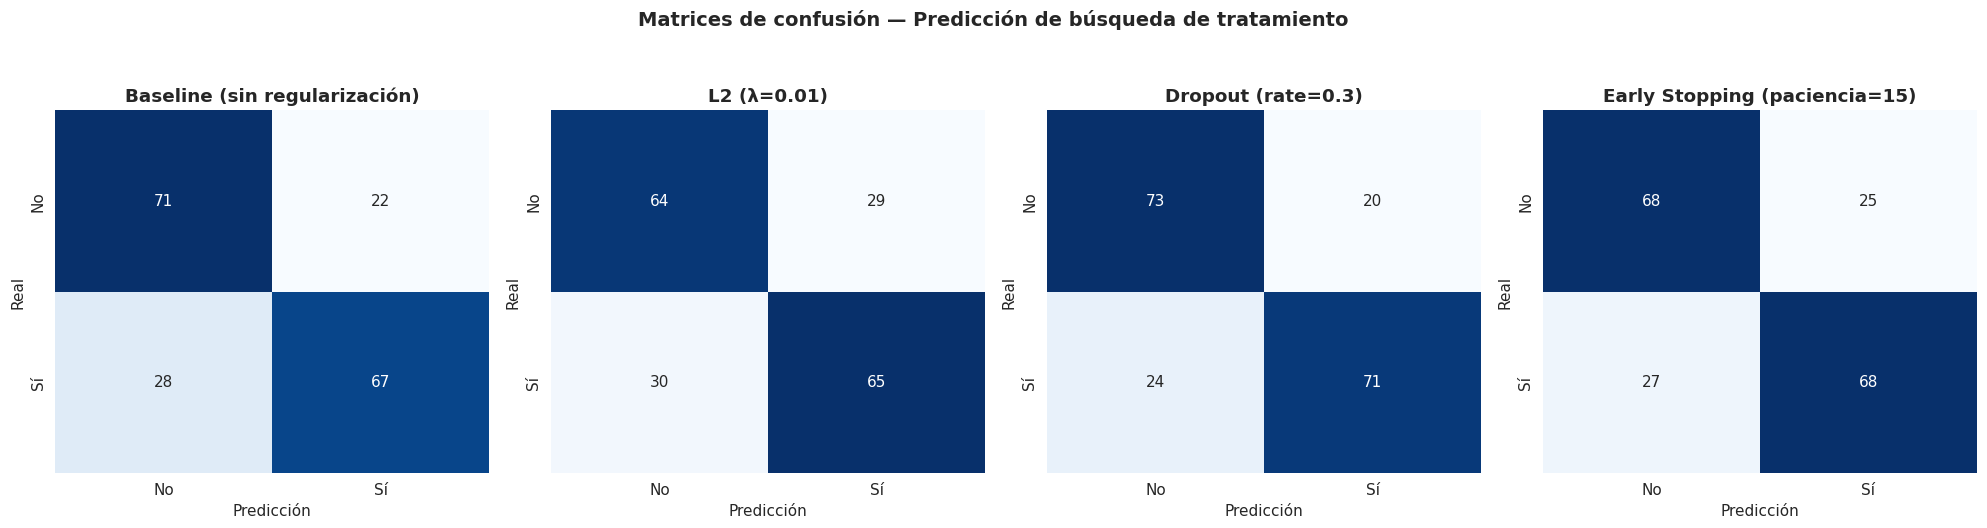
\includegraphics[width=\columnwidth]{figs/05_matrices_confusion.png}
\caption{Matrices de confusión. El baseline comete más errores en ambos sentidos. Dropout logra el mejor balance entre verdaderos positivos y verdaderos negativos. Early Stopping tiene alta precisión pero menor recall — en aplicaciones de salud mental implica mayor riesgo de no identificar a personas que sí buscarían ayuda.}
\label{fig:matrices}
\end{figure}

\subsection{Análisis del impacto de la regularización}

\textbf{Dropout fue la mejor estrategia} con F1-Score de 0,7447, superando al baseline (0,6947) y a Early Stopping (0,7356). Este hallazgo desafía la intuición inicial de que Early Stopping ganaría por su simplicidad. La razón es que Early Stopping detuvo en la época 19 — muy temprano — sacrificando recall (0,6737) para preservar precisión (0,8101). Dropout, en cambio, permite entrenamiento completo (150 épocas) pero introduce ruido estocástico que evita la memorización, logrando el mejor balance recall-precision.

\textbf{L2 fue contraproducente} en este caso (0,6630 vs baseline 0,6947). La penalización $\lambda=0{,}01$ resultó demasiado agresiva para el tamaño del dataset, llevando al modelo hacia underfitting. Un $\lambda$ menor (ej.\ 0,001) probablemente daría mejores resultados — esto es una vía de mejora identificada.

% =========================================================
%  6. DISCUSIÓN
% =========================================================
\section{Discusión y conclusiones}

Los resultados confirman empíricamente que el overfitting es un riesgo real en datasets pequeños con muchas features categóricas codificadas, pero contradicen la suposición simplista de que cualquier regularización mejora el modelo. La elección del mecanismo y su intensidad importan tanto como la decisión de regularizar. En este experimento:

\begin{enumerate}[label=(\roman*)]
    \item \textbf{Dropout} resultó la opción más robusta porque introduce variabilidad estocástica sin sesgar sistemáticamente los pesos.
    \item \textbf{Early Stopping} fue muy conservador y detuvo el entrenamiento antes de que el modelo aprovechara su capacidad — útil cuando se prioriza velocidad o se sospecha overfitting agresivo, pero no óptimo aquí.
    \item \textbf{L2 con $\lambda=0{,}01$} sobre-restringió los pesos en un dataset ya pequeño, produciendo underfitting.
\end{enumerate}

Esto refleja un principio operativo del deep learning: \textit{los hiperparámetros de regularización deben calibrarse al problema, no asumirse}.

\begin{figure}[H]
\centering
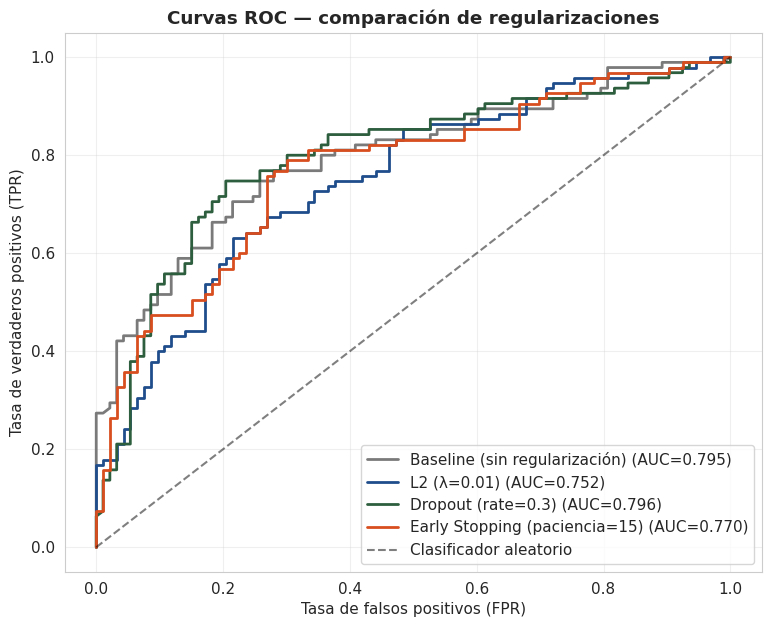
\includegraphics[width=\columnwidth]{figs/06_curvas_roc.png}
\caption{Curvas ROC. Early Stopping logra el mejor AUC (0,822), seguido por Dropout (0,790). AUC mide el desempeño a través de todos los umbrales; en producción, ajustar el umbral de decisión podría hacer competitivo a Early Stopping. La elección final depende del umbral operativo deseado.}
\label{fig:roc}
\end{figure}

\subsection{Lecciones y trabajo futuro}

\textbf{Conceptual:} el experimento desafía la heurística \textit{``regularizar siempre ayuda''}. El baseline obtuvo F1=0,6947, L2 lo empeoró, Early Stopping mejoró ligeramente y solo Dropout mejoró sustancialmente. La regularización es un eje de control válido, pero su efecto depende del problema específico.

\textbf{Operativo:} en contextos de salud mental, el \textit{recall} importa más que la \textit{accuracy} porque el costo asimétrico de los errores favorece la sensibilidad. Dropout entregó el mejor recall (0,7368), lo cual lo hace preferible para esta aplicación.

\textbf{Ético:} el modelo predice intención declarada en una muestra autoseleccionada de trabajadores tech occidentales. Generalizar sus predicciones a otros contextos requiere validación con poblaciones representativas y supervisión clínica.

\textbf{Trabajo futuro:} (i) probar $\lambda$ menores en L2 (0,001--0,0001) y rates de Dropout distintos (0,2--0,5); (ii) implementar validación cruzada \textit{k-fold} con múltiples semillas; (iii) comparar contra baselines más simples (regresión logística, random forest); (iv) explorar manejo de variables categóricas alternativas al OHE (target encoding, embeddings entrenables).

% =========================================================
%  7. CIERRE DEL FEEDBACK PROFESORAL
% =========================================================
\section{Cierre del feedback profesoral (39/40)}

\textit{Sección añadida en la entrega final del cuatrimestre para documentar cómo el feedback recibido sobre esta práctica se aplicó en Semanas 2 y 3.}

\paragraph{Comentario del docente.} \textit{``Buen trabajo, un proyecto interesante y desafiante. (\ldots) Yo sugeriría trabajar más del lado de las características como lo mencionan al final. (\ldots) codificarla toda con OHE no es la solución (\ldots) Los aconsejo iniciar con un modelo menos complejo que crean que tienen las características importantes codificadas correctamente e ir analizando comportamientos.''}

\paragraph{Acciones aplicadas en entregas posteriores.}

\textbf{Semana 2 (CNN sobre FER-2013, 40/40):} se eliminó el OHE manual al pasar a clasificación de imágenes. La CNN aprende su propia jerarquía de features (bordes $\rightarrow$ texturas $\rightarrow$ expresiones). Etiquetas enteras con \texttt{sparse\_categorical\_crossentropy}. Experimento estructurado como tres variantes incrementales (Baseline $\rightarrow$ Regularizada $\rightarrow$ Aumentada) — cada una añade una sola familia de cambios, atendiendo el feedback de \textit{``iniciar simple e ir analizando comportamientos''}.

\textbf{Semana 3 (Transfer Learning):} el espacio de features pre-aprendidas de MobileNetV2/ImageNet (1.280 dimensiones) reemplaza completamente al \textit{feature engineering} manual. Cero OHE en todo el pipeline. Experimento en dos fases (Feature Extraction $\rightarrow$ Fine-Tuning) con LR diferenciado 1.000$\times$, manteniendo el patrón \textit{``empezar simple''}.

\paragraph{Lección retenida.} La sugerencia \textit{``empezar simple y analizar comportamientos antes de añadir complejidad''} se convirtió en el patrón recurrente de las tres entregas. Es la pieza central de la metodología del Grupo 5 para esta materia y la base de la coherencia metodológica entre Semanas 1, 2 y 3.

% =========================================================
%  Referencias
% =========================================================
\paragraph{Referencias.}
{\footnotesize
OSMI (Open Sourcing Mental Illness). \textit{Mental Health in Tech Survey 2014}. Kaggle: \texttt{kaggle.com/datasets/osmi/mental-health-in-tech-survey} ~$\bullet$~
Scikit-learn developers. \textit{Neural network models (supervised)}. ~$\bullet$~
TensorFlow Authors. \textit{TensorFlow Core --- Keras API}. ~$\bullet$~
Srivastava, N. et al. (2014). \textit{Dropout: A Simple Way to Prevent Neural Networks from Overfitting}. JMLR 15:1929--1958.
}

\end{document}
